\cleardoublepage
\chapter{Solução} \label{capituloSolucoes}

Neste capítulo iremos explorar a solução encontrada para os vários desafios e necessidades encontradas ao longo desta dissertação.

\section{Autenticação local}

\subsection{Especificação} \label{especificacaoAuthLocal}

De modo a satisfazer as necessidades da autenticação local de utilizadores, através de username e password, foi decidida a implementação de uma base de dados em \emph{MongoDB}.

A criação de um utilizador na plataforma \gls{clav} obriga ao preenchimento dos seguintes dados:

\begin{enumerate}
    \item \textbf{Nome}
    
        Qualquer combinação de números e letras.
    \item \textbf{Email}
    
        Considera-se um email válido qualquer combinação de letras e números, seguida de um "@" com terminação em "." seguido de letras.
    \item \textbf{Nível de utilizador}
    
        Durante a fase de registo é obrigatória a seleção do nível de utilizador do mesmo, sendo esta utilizada para verificação de nível de acesso dentro da plataforma \gls{clav}.
    \begin{enumerate}
        \item Administrador de Perfil Tecnológico
        \item Administrador de Perfil Funcional
        \item Utilizador Validador
        \item Utilizador Avançado
        \item Utilizador Decisor
        \item Utilizador Simples
        \item Representante Entidade
    \end{enumerate}
    \item \textbf{Entidade}
    
        A escolha de uma entidade ao qual o utilizador pertence é de caratér obrigatório, não sendo permitido o registo sem a mesma ser selecionada. Para tal efeito, é carregada uma lista com centenas de entidades das quais o utilizador escolherá uma.
        
    \item \textbf{Password}
    
        Qualquer combinação de números e letras.
\end{enumerate}

Além da obrigatoriedade dos dados prévios, foi também decidido que todos os dados relativos aos utilizadores iriam ser guardados numa coleção MongoDB com o nome "\emph{users}".

\subsection{Workflow da autenticação}

\begin{figure}[h]
    \centering
    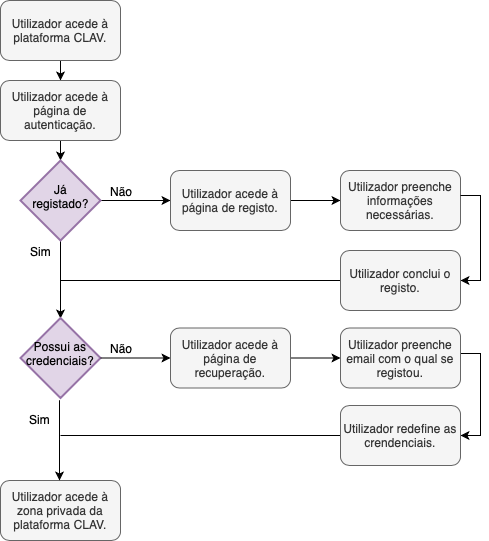
\includegraphics[width=0.725\textwidth]{img/diagramas/authlocal/AuthLocal.png}
    \caption{Workflow da autenticação local.}
    \label{fig:flow_authlocal}
\end{figure}

\cleardoublepage
\section{Autenticação através de Cartão de Cidadão}
\subsection{Especificação}

A autenticação através de Cartão de Cidadão é baseada na autenticação local, havendo distinção entre os utilizadores registados via username e password, e aqueles registados através de Cartão de Cidadão.

\begin{enumerate}
    \item \textbf{Nome}
    
        Qualquer combinação de números e letras.
    \item \textbf{Email}
    
        Considera-se um email válido qualquer combinação de letras e números, seguida de um "@" com terminação em "." seguido de letras.
    \item \textbf{Nível de utilizador}
    
        Durante a fase de registo é obrigatória a seleção do nível de utilizador do mesmo, sendo esta utilizada para verificação de nível de acesso dentro da plataforma \gls{clav}.
    \begin{enumerate}
        \item Administrador de Perfil Tecnológico
        \item Administrador de Perfil Funcional
        \item Utilizador Validador
        \item Utilizador Avançado
        \item Utilizador Decisor
        \item Utilizador Simples
        \item Representante Entidade
    \end{enumerate}
    \item \textbf{Entidade}
    
        A escolha de uma entidade ao qual o utilizador pertence é de caratér obrigatório, não sendo permitido o registo sem a mesma ser selecionada.
\end{enumerate}

\cleardoublepage
\subsection{Workflow da autenticação}

\begin{figure}[h!]
    \centering
    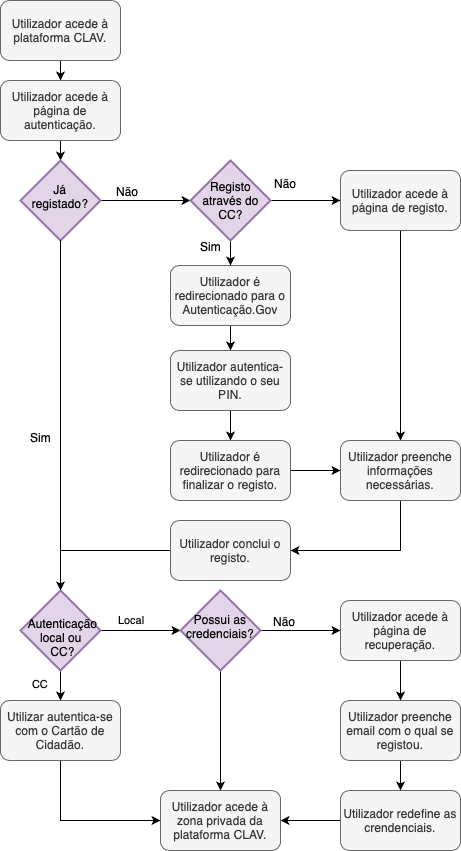
\includegraphics[width=0.695\textwidth]{img/diagramas/authCC/AuthCC.png}
    \caption{Workflow da autenticação através de Cartão de Cidadão.}
    \label{fig:flow_authCC}
\end{figure}

\cleardoublepage
\section{Proteção da API de dados}

\subsection{Especificação}

De modo a fornecer uma camada de proteção à \gls{api} de dados, é necessário identificar e autenticar os pedidos que a ela chegam.

Para tal, a solução encontrada foi a implementação de duas funções de middleware responsáveis pela seguinte função:

\begin{enumerate}
    \item \textbf{Verificação da origem do pedido}
    
    Função de middleware cujo funcionamento é baseado em tokens \gls{jwt}. Esta função é executada sempre que há um pedido à \gls{api} e verifica se o pedido obedece aos seguintes critérios:

    \begin{enumerate}
        \item \textbf{Presença do token}
        
        Todo e qualquer pedido à \gls{api} de dados da plataforma \gls{clav}, seja um \emph{GET}, \emph{POST}, entre outros, tem de ser enviado com um token baseado em \gls{jwt}.
        
        \item \textbf{Validade do token}
        
        Após receção do token, este irá ser descodificado e irá ocorrer a verificação da validade do mesmo, ou seja, se o token é válido e contem o identificador do utilizador que fez o pedido à API.
    \end{enumerate}
    
    \item \textbf{Verificação do nível de acesso}
    
    Caso o token seja válido e de facto contem o identificador do utilizador, é verificado o nível de acesso do mesmo. Caso este esteja a tentar aceder a funções da \gls{api} que necessitam de um nível superior ao fornecido, o pedido é negado, caso contrário é permitido o acesso à informação pedida. 
\end{enumerate}

\cleardoublepage
\subsection{Workflow da autenticação}

\begin{figure}[h!]
    \centering
    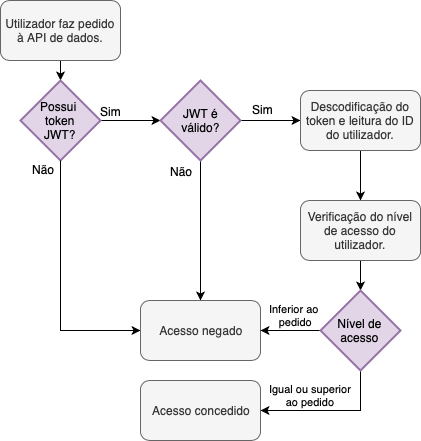
\includegraphics[width=\textwidth]{img/diagramas/authAPI/AuthAPI.png}
    \caption{Workflow da autenticação de pedidos à API de dados.}
    \label{fig:flow_authCC}
\end{figure}

\cleardoublepage
\section{Gestão de utilizadores}

\cleardoublepage
\section{Métrica da plataforma}